% Options for packages loaded elsewhere
\PassOptionsToPackage{unicode}{hyperref}
\PassOptionsToPackage{hyphens}{url}
\PassOptionsToPackage{dvipsnames,svgnames,x11names}{xcolor}
%
\documentclass[
  12pt,
  letterpaper,
]{book}

\usepackage{amsmath,amssymb}
\usepackage{iftex}
\ifPDFTeX
  \usepackage[T1]{fontenc}
  \usepackage[utf8]{inputenc}
  \usepackage{textcomp} % provide euro and other symbols
\else % if luatex or xetex
  \usepackage{unicode-math}
  \defaultfontfeatures{Scale=MatchLowercase}
  \defaultfontfeatures[\rmfamily]{Ligatures=TeX,Scale=1}
\fi
\usepackage{lmodern}
\ifPDFTeX\else  
    % xetex/luatex font selection
\fi
% Use upquote if available, for straight quotes in verbatim environments
\IfFileExists{upquote.sty}{\usepackage{upquote}}{}
\IfFileExists{microtype.sty}{% use microtype if available
  \usepackage[]{microtype}
  \UseMicrotypeSet[protrusion]{basicmath} % disable protrusion for tt fonts
}{}
\makeatletter
\@ifundefined{KOMAClassName}{% if non-KOMA class
  \IfFileExists{parskip.sty}{%
    \usepackage{parskip}
  }{% else
    \setlength{\parindent}{0pt}
    \setlength{\parskip}{6pt plus 2pt minus 1pt}}
}{% if KOMA class
  \KOMAoptions{parskip=half}}
\makeatother
\usepackage{xcolor}
\usepackage[margin=1in]{geometry}
\setlength{\emergencystretch}{3em} % prevent overfull lines
\setcounter{secnumdepth}{5}
% Make \paragraph and \subparagraph free-standing
\makeatletter
\ifx\paragraph\undefined\else
  \let\oldparagraph\paragraph
  \renewcommand{\paragraph}{
    \@ifstar
      \xxxParagraphStar
      \xxxParagraphNoStar
  }
  \newcommand{\xxxParagraphStar}[1]{\oldparagraph*{#1}\mbox{}}
  \newcommand{\xxxParagraphNoStar}[1]{\oldparagraph{#1}\mbox{}}
\fi
\ifx\subparagraph\undefined\else
  \let\oldsubparagraph\subparagraph
  \renewcommand{\subparagraph}{
    \@ifstar
      \xxxSubParagraphStar
      \xxxSubParagraphNoStar
  }
  \newcommand{\xxxSubParagraphStar}[1]{\oldsubparagraph*{#1}\mbox{}}
  \newcommand{\xxxSubParagraphNoStar}[1]{\oldsubparagraph{#1}\mbox{}}
\fi
\makeatother

\usepackage{color}
\usepackage{fancyvrb}
\newcommand{\VerbBar}{|}
\newcommand{\VERB}{\Verb[commandchars=\\\{\}]}
\DefineVerbatimEnvironment{Highlighting}{Verbatim}{commandchars=\\\{\}}
% Add ',fontsize=\small' for more characters per line
\usepackage{framed}
\definecolor{shadecolor}{RGB}{241,243,245}
\newenvironment{Shaded}{\begin{snugshade}}{\end{snugshade}}
\newcommand{\AlertTok}[1]{\textcolor[rgb]{0.68,0.00,0.00}{#1}}
\newcommand{\AnnotationTok}[1]{\textcolor[rgb]{0.37,0.37,0.37}{#1}}
\newcommand{\AttributeTok}[1]{\textcolor[rgb]{0.40,0.45,0.13}{#1}}
\newcommand{\BaseNTok}[1]{\textcolor[rgb]{0.68,0.00,0.00}{#1}}
\newcommand{\BuiltInTok}[1]{\textcolor[rgb]{0.00,0.23,0.31}{#1}}
\newcommand{\CharTok}[1]{\textcolor[rgb]{0.13,0.47,0.30}{#1}}
\newcommand{\CommentTok}[1]{\textcolor[rgb]{0.37,0.37,0.37}{#1}}
\newcommand{\CommentVarTok}[1]{\textcolor[rgb]{0.37,0.37,0.37}{\textit{#1}}}
\newcommand{\ConstantTok}[1]{\textcolor[rgb]{0.56,0.35,0.01}{#1}}
\newcommand{\ControlFlowTok}[1]{\textcolor[rgb]{0.00,0.23,0.31}{\textbf{#1}}}
\newcommand{\DataTypeTok}[1]{\textcolor[rgb]{0.68,0.00,0.00}{#1}}
\newcommand{\DecValTok}[1]{\textcolor[rgb]{0.68,0.00,0.00}{#1}}
\newcommand{\DocumentationTok}[1]{\textcolor[rgb]{0.37,0.37,0.37}{\textit{#1}}}
\newcommand{\ErrorTok}[1]{\textcolor[rgb]{0.68,0.00,0.00}{#1}}
\newcommand{\ExtensionTok}[1]{\textcolor[rgb]{0.00,0.23,0.31}{#1}}
\newcommand{\FloatTok}[1]{\textcolor[rgb]{0.68,0.00,0.00}{#1}}
\newcommand{\FunctionTok}[1]{\textcolor[rgb]{0.28,0.35,0.67}{#1}}
\newcommand{\ImportTok}[1]{\textcolor[rgb]{0.00,0.46,0.62}{#1}}
\newcommand{\InformationTok}[1]{\textcolor[rgb]{0.37,0.37,0.37}{#1}}
\newcommand{\KeywordTok}[1]{\textcolor[rgb]{0.00,0.23,0.31}{\textbf{#1}}}
\newcommand{\NormalTok}[1]{\textcolor[rgb]{0.00,0.23,0.31}{#1}}
\newcommand{\OperatorTok}[1]{\textcolor[rgb]{0.37,0.37,0.37}{#1}}
\newcommand{\OtherTok}[1]{\textcolor[rgb]{0.00,0.23,0.31}{#1}}
\newcommand{\PreprocessorTok}[1]{\textcolor[rgb]{0.68,0.00,0.00}{#1}}
\newcommand{\RegionMarkerTok}[1]{\textcolor[rgb]{0.00,0.23,0.31}{#1}}
\newcommand{\SpecialCharTok}[1]{\textcolor[rgb]{0.37,0.37,0.37}{#1}}
\newcommand{\SpecialStringTok}[1]{\textcolor[rgb]{0.13,0.47,0.30}{#1}}
\newcommand{\StringTok}[1]{\textcolor[rgb]{0.13,0.47,0.30}{#1}}
\newcommand{\VariableTok}[1]{\textcolor[rgb]{0.07,0.07,0.07}{#1}}
\newcommand{\VerbatimStringTok}[1]{\textcolor[rgb]{0.13,0.47,0.30}{#1}}
\newcommand{\WarningTok}[1]{\textcolor[rgb]{0.37,0.37,0.37}{\textit{#1}}}

\providecommand{\tightlist}{%
  \setlength{\itemsep}{0pt}\setlength{\parskip}{0pt}}\usepackage{longtable,booktabs,array}
\usepackage{calc} % for calculating minipage widths
% Correct order of tables after \paragraph or \subparagraph
\usepackage{etoolbox}
\makeatletter
\patchcmd\longtable{\par}{\if@noskipsec\mbox{}\fi\par}{}{}
\makeatother
% Allow footnotes in longtable head/foot
\IfFileExists{footnotehyper.sty}{\usepackage{footnotehyper}}{\usepackage{footnote}}
\makesavenoteenv{longtable}
\usepackage{graphicx}
\makeatletter
\def\maxwidth{\ifdim\Gin@nat@width>\linewidth\linewidth\else\Gin@nat@width\fi}
\def\maxheight{\ifdim\Gin@nat@height>\textheight\textheight\else\Gin@nat@height\fi}
\makeatother
% Scale images if necessary, so that they will not overflow the page
% margins by default, and it is still possible to overwrite the defaults
% using explicit options in \includegraphics[width, height, ...]{}
\setkeys{Gin}{width=\maxwidth,height=\maxheight,keepaspectratio}
% Set default figure placement to htbp
\makeatletter
\def\fps@figure{htbp}
\makeatother
% definitions for citeproc citations
\NewDocumentCommand\citeproctext{}{}
\NewDocumentCommand\citeproc{mm}{%
  \begingroup\def\citeproctext{#2}\cite{#1}\endgroup}
\makeatletter
 % allow citations to break across lines
 \let\@cite@ofmt\@firstofone
 % avoid brackets around text for \cite:
 \def\@biblabel#1{}
 \def\@cite#1#2{{#1\if@tempswa , #2\fi}}
\makeatother
\newlength{\cslhangindent}
\setlength{\cslhangindent}{1.5em}
\newlength{\csllabelwidth}
\setlength{\csllabelwidth}{3em}
\newenvironment{CSLReferences}[2] % #1 hanging-indent, #2 entry-spacing
 {\begin{list}{}{%
  \setlength{\itemindent}{0pt}
  \setlength{\leftmargin}{0pt}
  \setlength{\parsep}{0pt}
  % turn on hanging indent if param 1 is 1
  \ifodd #1
   \setlength{\leftmargin}{\cslhangindent}
   \setlength{\itemindent}{-1\cslhangindent}
  \fi
  % set entry spacing
  \setlength{\itemsep}{#2\baselineskip}}}
 {\end{list}}
\usepackage{calc}
\newcommand{\CSLBlock}[1]{\hfill\break\parbox[t]{\linewidth}{\strut\ignorespaces#1\strut}}
\newcommand{\CSLLeftMargin}[1]{\parbox[t]{\csllabelwidth}{\strut#1\strut}}
\newcommand{\CSLRightInline}[1]{\parbox[t]{\linewidth - \csllabelwidth}{\strut#1\strut}}
\newcommand{\CSLIndent}[1]{\hspace{\cslhangindent}#1}

% header.tex
\usepackage{xcolor}        % Para colores
\usepackage{polyglossia}   % Soporte de idiomas con XeLaTeX
\setdefaultlanguage{spanish}

% Definición de colores personalizados
\definecolor{fecundidad}{HTML}{FFC125}      % Amarillo
\definecolor{supervivencia}{HTML}{36648B}   % Azul
\definecolor{crecimiento}{HTML}{548B54}     % Verde
\definecolor{retroceso}{HTML}{7A378B}       % Violeta
\definecolor{permanencia}{HTML}{26466A}     % Azul oscuro
\usepackage{booktabs}
\usepackage{caption}
\usepackage{longtable}
\usepackage{colortbl}
\usepackage{array}
\usepackage{anyfontsize}
\usepackage{multirow}
\makeatletter
\@ifpackageloaded{caption}{}{\usepackage{caption}}
\AtBeginDocument{%
\ifdefined\contentsname
  \renewcommand*\contentsname{Table of contents}
\else
  \newcommand\contentsname{Table of contents}
\fi
\ifdefined\listfigurename
  \renewcommand*\listfigurename{List of Figures}
\else
  \newcommand\listfigurename{List of Figures}
\fi
\ifdefined\listtablename
  \renewcommand*\listtablename{List of Tables}
\else
  \newcommand\listtablename{List of Tables}
\fi
\ifdefined\figurename
  \renewcommand*\figurename{Figure}
\else
  \newcommand\figurename{Figure}
\fi
\ifdefined\tablename
  \renewcommand*\tablename{Table}
\else
  \newcommand\tablename{Table}
\fi
}
\@ifpackageloaded{float}{}{\usepackage{float}}
\floatstyle{ruled}
\@ifundefined{c@chapter}{\newfloat{codelisting}{h}{lop}}{\newfloat{codelisting}{h}{lop}[chapter]}
\floatname{codelisting}{Listing}
\newcommand*\listoflistings{\listof{codelisting}{List of Listings}}
\makeatother
\makeatletter
\makeatother
\makeatletter
\@ifpackageloaded{caption}{}{\usepackage{caption}}
\@ifpackageloaded{subcaption}{}{\usepackage{subcaption}}
\makeatother

\ifLuaTeX
  \usepackage{selnolig}  % disable illegal ligatures
\fi
\usepackage{bookmark}

\IfFileExists{xurl.sty}{\usepackage{xurl}}{} % add URL line breaks if available
\urlstyle{same} % disable monospaced font for URLs
\hypersetup{
  colorlinks=true,
  linkcolor={Maroon},
  filecolor={Maroon},
  citecolor={Blue},
  urlcolor={Blue},
  pdfcreator={LaTeX via pandoc}}


\author{}
\date{}

\begin{document}
\frontmatter

\renewcommand*\contentsname{Table of contents}
{
\hypersetup{linkcolor=}
\setcounter{tocdepth}{2}
\tableofcontents
}

\mainmatter
\chapter{Dinámica transitoria}\label{Dinamica_transitoria}

Autores: ``Mariana Hernández Apolinar, Tamara Ticktin y Paola Portillo
Tzompa''

\subsubsection{Librerías de R requeridas para el siguiente
módulo}\label{libreruxedas-de-r-requeridas-para-el-siguiente-muxf3dulo}

\begin{Shaded}
\begin{Highlighting}[]
\DocumentationTok{\#\# Librerías de R requeridas para el análisis}

\FunctionTok{library}\NormalTok{(popdemo)}
\FunctionTok{library}\NormalTok{(popbio)}
\FunctionTok{library}\NormalTok{(ggplot2)}
\FunctionTok{library}\NormalTok{(dplyr)}
\FunctionTok{library}\NormalTok{(scales)}
\FunctionTok{library}\NormalTok{(tidyverse)}
\FunctionTok{library}\NormalTok{(gt)}
\end{Highlighting}
\end{Shaded}

\section{Dinámica poblacional de largo y corto
plazo}\label{dinuxe1mica-poblacional-de-largo-y-corto-plazo}

Los modelos de proyección poblacional (MPP), previamente abordados en el
capítulo de Índices, constituyen las herramientas más empleadas para
estimar el crecimiento futuro de una población (i.e., largo plazo).
Estos modelos suelen asumir la constancia en las tasas vitales
---proporciones de mortalidad, reproducción y crecimiento de los
individuos en las distintas categorías poblacionales--- bajo condiciones
ambientales invariables (Caswell, 1989; Crone et al., 2011; Koons, Iles
\& Stott, 2021). En ausencia de variación (i.e., modelos deterministas),
se espera que la población crezca o decrezca a una velocidad constante,
denominada tasa finita o asintótica de crecimiento poblacional (\(λ\))
(Caswell, 1989; Bierzychudek, 1999). Este patrón estable se alcanza
cuando la proporción de individuos por categoría de tamaño o estado
permanece constante, condición conocida como estructura estable (\(w\)).

Sin embargo, en sistemas naturales las condiciones poblacionales y
ambientales rara vez son constantes. Las poblaciones enfrentan recursos
limitados (e.g., alimento, refugio), ambientes heterogéneos y
perturbaciones (e.g., deforestación, sequías, huracanes, enfermedades),
que alteran su dinámica y evidencian que la tasa de crecimiento a largo
plazo (\(λ\)) no siempre predice adecuadamente los cambios poblacionales
(Bierzychudek, 1999). Por ello, se han desarrollado modelos que
incorporan variabilidad ambiental y permiten proyecciones más realistas,
como los modelos estocásticos (ver capítulo 10) y los análisis de
dinámica transitoria.

\section{Modelos de dinámica
transitoria}\label{modelos-de-dinuxe1mica-transitoria}

Los modelos de dinámica transitoria se proponen como alternativa para
evaluar la respuesta poblacional ante perturbaciones súbitas de origen
biótico (e.g., depredación), abiótico (e.g., huracán) o antropogénico
(e.g., extracción) (Ezard et al., 2010). Una característica distintiva
es que el disturbio afecta únicamente la estructura poblacional, sin
modificar los valores de la matriz de transición, que permanecen
constantes en el tiempo (Stott, Townley \& Hodgson, 2011; Vindenes et
al., 2021). Este cambio abrupto genera una respuesta instantánea,
temporal y de corto plazo, generalmente distinta a la dinámica esperada
en el largo plazo (Ezard et al., 2010; Stott et al., 2010; Koons, Iles
\& Stott, 2021).

Para comprender cómo la estructura inicial influye en el crecimiento
poblacional, estos modelos asumen una estructura inestable, lo que
permite analizar la respuesta antes de alcanzar el crecimiento
asintótico (i.e., \(λ\) constante y estructura estable) (Bierzychudek,
1999; Stott, Townley \& Hodgson, 2011; Stott, Hodgson \& Townley, 2012a;
Koons, Iles \& Stott, 2021). La respuesta se evalúa mediante las
discrepancias entre el comportamiento poblacional bajo una o varias
estructuras iniciales (corto plazo) y la estructura estable (largo
plazo) (Raventós et al., 2015). Dichas diferencias se reflejan en
incrementos (ampliación), decrementos (atenuación) o fluctuaciones en la
abundancia poblacional a corto plazo respecto al largo plazo (Stott,
Townley \& Hodgson, 2011), cuantificadas mediante los índices de
transferencia (Stott, Townley \& Hodgson, 2011).

Actualmente, los modelos de dinámica transitoria han demostrado ser
herramientas valiosas en estudios poblacionales de orquídeas, ya que
permiten evaluar estrategias de conservación y manejo (Raventós et al.,
2015; Tremblay, Raventos \& Ackerman, 2015; Ospina-Calderón et al.,
2023). Aunque estos análisis existen desde hace décadas (Crone et al.,
2011), su accesibilidad aumentó significativamente a partir de 2010
(Stott, Hodgson \& Townley, 2012b).

El marco metodológico propuesto por Stott y colaboradores (Stott,
Townley \& Hodgson, 2011; Stott, Hodgson \& Townley, 2012b; Stott,
Hodgson \& Townley, 2012a) incluye procedimientos matemáticos
implementados en el software estadístico R, que facilitan el cálculo y
análisis de la dinámica transitoria. Para desarrollar un proyecto de
este tipo, se recomienda seguir los pasos resumidos a continuación:

\subsection{Procedimiento básicos}\label{procedimiento-buxe1sicos}

\begin{enumerate}
\def\labelenumi{\arabic{enumi})}
\tightlist
\item
  \textbf{Análisis de la dinámica de largo plazo}
\end{enumerate}

\begin{itemize}
\tightlist
\item
  Construcción de la matriz de transición y definición de la estructura
  inicial.
\item
  Estimación del crecimiento asintótico (\(λ\)).
\end{itemize}

\begin{enumerate}
\def\labelenumi{\arabic{enumi})}
\setcounter{enumi}{1}
\tightlist
\item
  \textbf{Análisis de la dinámica de corto plazo}
\end{enumerate}

\begin{itemize}
\tightlist
\item
  Definición de la estructura poblacional inicial.
\item
  Evaluación de la dinámica absoluta.
\item
  Dinámica transitoria estandarizada.
\item
  Cálculo de límites transitorios.
\end{itemize}

Cabe destacar que los modelos de dinámica transitoria constituyen la
única herramienta para evaluar poblaciones que nunca convergen ---o cuya
convergencia es improbable--- hacia una estructura estable (Hinrichsen,
2025).

\begin{center}\rule{0.5\linewidth}{0.5pt}\end{center}

\section{Proyecto de dinámica transitoria o de corto
plazo}\label{proyecto-de-dinuxe1mica-transitoria-o-de-corto-plazo}

\subsection{Análisis de la dinámica de largo
plazo}\label{anuxe1lisis-de-la-dinuxe1mica-de-largo-plazo}

Como punto de partida y con la finalidad de contrastar su comportamiento
con el de corto plazo, se describe el crecimiento de la población a
largo plazo: tasas vitales constantes y en condiciones ambientales sin
variación.

\begin{enumerate}
\def\labelenumi{\alph{enumi})}
\tightlist
\item
  \emph{Matriz de transición y estructura poblacional inicial}. Para
  estimar el crecimiento futuro de la población se debe de contar con la
  matriz de proyección poblacional y su correspondiente vector de la
  estructura poblacional observada al inicio del estudio de una o varias
  poblaciones. En el análisis se usarán los datos obtenidos para
  \emph{Lepanthes rubripetala}, una orquídea epífita miniatura, endémica
  de Puerto Rico. Tremblay y colaboradores (Tremblay, Raventos \&
  Ackerman, 2015) analizaron mensualmente seis poblaciones de la especie
  de junio de 1994 a enero de 1996. En específico en este capítulo
  usaremos la matriz promedio de la población 1 (Tremblay, Raventos \&
  Ackerman, 2015) y su correspondiente estructura poblacional
  (Schödelbauerová, Tremblay \& Kindlmann, 2010).
\end{enumerate}

\begin{figure}[H]

{\centering 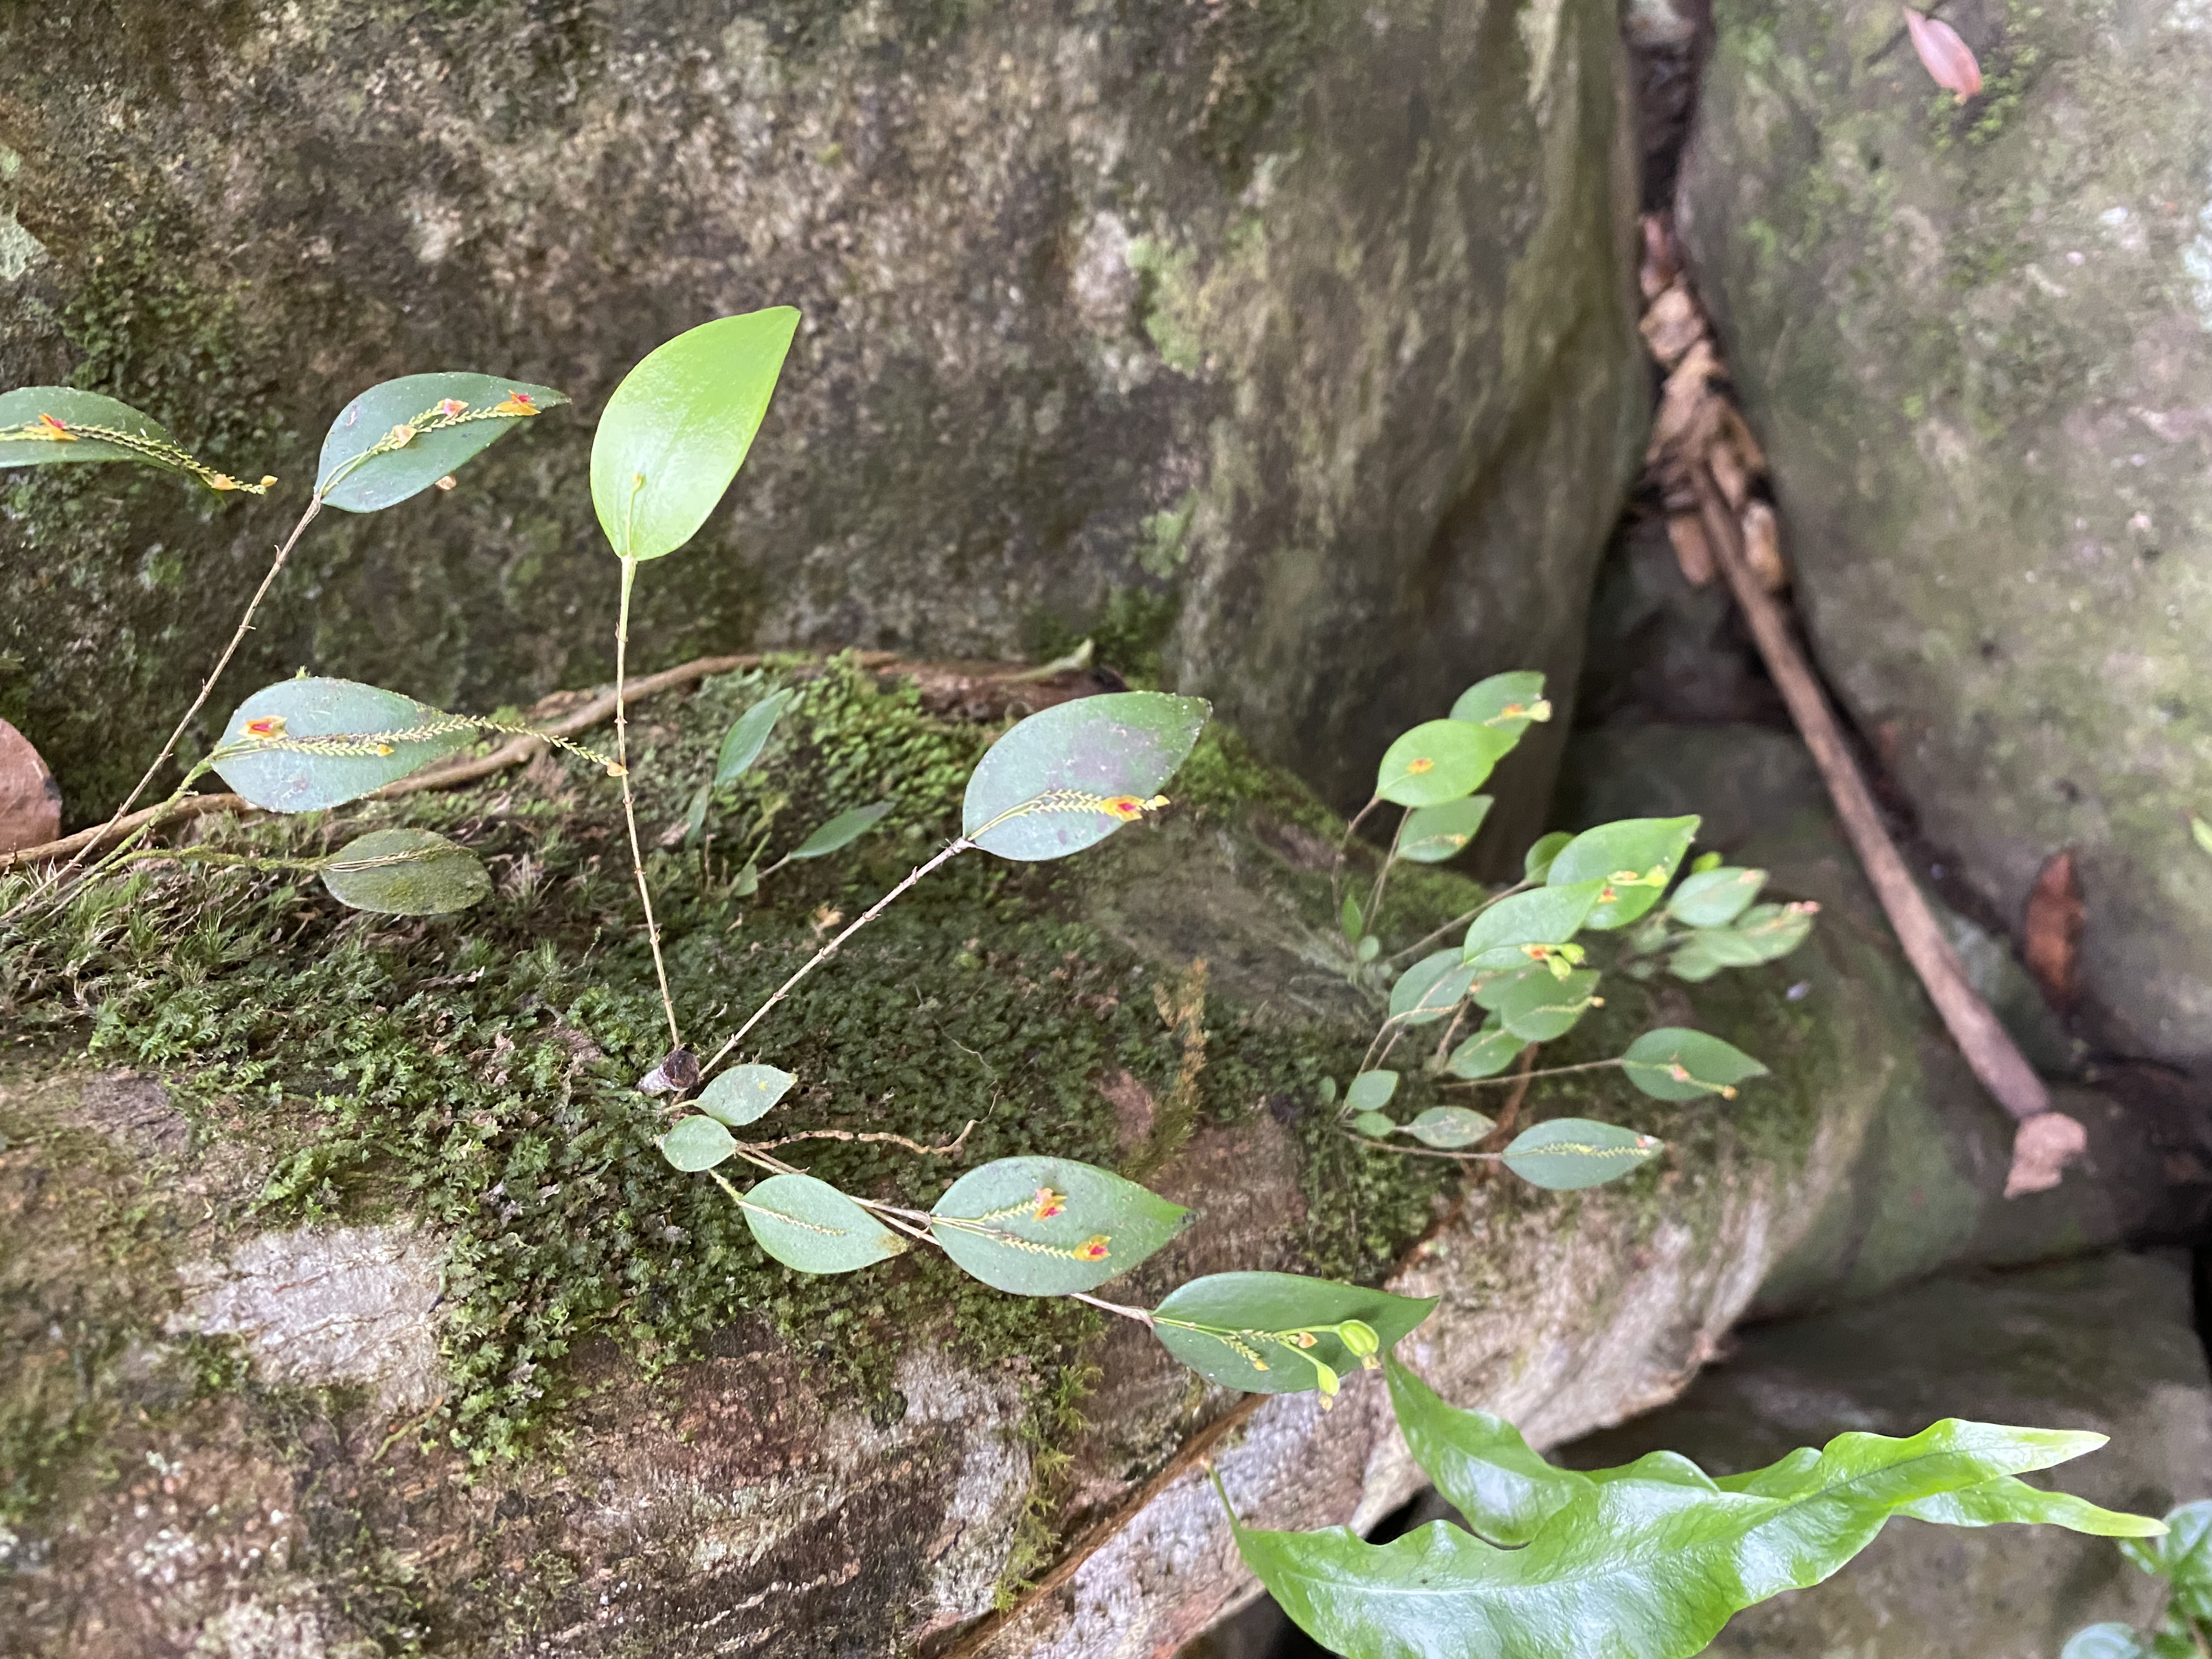
\includegraphics{Species/Lepanthes rupestris Tremblay.jpeg}

}

\caption{\emph{Lepanthes rupestris}. Foto: Tremblay}

\end{figure}%

El ciclo de vida de \emph{L. rubripetala} fue dividido en cuatro
categorías de estado: plántula (PL), juvenil (J), adulto no reproductivo
(NR) y adulto reproductivo (AR). Esta última categoría florece y produce
frutos a largo de todo el año (Schödelbauerová, Tremblay \& Kindlmann,
2010; Tremblay, Raventos \& Ackerman, 2015). En consecuencia, la
estructura poblacional cuenta con una columna de 4 elementos, que
indican el número de individuos encontrado en el estado de plántula (0),
juvenil (46), adulto no reproductivo (38) y adulto reproductivo (82) al
inicio del estudio, indicado como \(t_{0}\) (Schödelbauerová, Tremblay
\& Kindlmann, 2010). Por su parte, la matriz de transición de \emph{L.
rubripetala} está formada por 4 renglones y 4 columnas (Tremblay,
Raventos \& Ackerman, 2015), que corresponden a los estados del ciclo de
vida de la especie y los 16 elementos de la probabilidad de permanencia,
transición a una categoría superior, retroceso a una categoría inferior
y fecundidad promedio por categoría (ver capítulo 5).

En el siguiente recuadro incorporamos la información de \emph{L.
rubripetala} en \emph{R}. La función \emph{matrix} fue usada para
construir la matriz de transición y \emph{n0} se usa para nombrar al
vector de la estructura inicial observada.

\begin{Shaded}
\begin{Highlighting}[]
\CommentTok{\#Capturar los datos de la matriz para L. rubripetala (Tremblay et al. 2015)}
\NormalTok{Lr1 }\OtherTok{\textless{}{-}} \FunctionTok{matrix}\NormalTok{(}\FunctionTok{c}\NormalTok{(}\FloatTok{0.4324}\NormalTok{, }\DecValTok{0}\NormalTok{,      }\DecValTok{0}\NormalTok{,     }\FloatTok{0.15}\NormalTok{,}
               \FloatTok{0.3784}\NormalTok{, }\FloatTok{0.8459}\NormalTok{, }\DecValTok{0}\NormalTok{,     }\DecValTok{0}\NormalTok{,}
               \DecValTok{0}\NormalTok{,      }\FloatTok{0.0034}\NormalTok{, }\FloatTok{0.7954}\NormalTok{,}\FloatTok{0.2300}\NormalTok{,}
               \DecValTok{0}\NormalTok{,      }\FloatTok{0.0890}\NormalTok{, }\FloatTok{0.1841}\NormalTok{,}\FloatTok{0.7510}\NormalTok{), }
      \AttributeTok{byrow=}\ConstantTok{TRUE}\NormalTok{,}\AttributeTok{ncol=}\DecValTok{4}\NormalTok{)}

\CommentTok{\#Capturar las categorias de estado}
\NormalTok{estadios }\OtherTok{\textless{}{-}} \FunctionTok{c}\NormalTok{(}\StringTok{"PL"}\NormalTok{, }\StringTok{"J"}\NormalTok{, }\StringTok{"NR"}\NormalTok{, }\StringTok{"AR"}\NormalTok{)}
\FunctionTok{colnames}\NormalTok{(Lr1) }\OtherTok{\textless{}{-}} \FunctionTok{rownames}\NormalTok{(Lr1) }\OtherTok{\textless{}{-}}\NormalTok{ estadios}

\CommentTok{\#Obtener la matriz L. rubripetala}
\NormalTok{Lr1 }\OtherTok{\textless{}{-}} \FunctionTok{matrix}\NormalTok{(Lr1[}\DecValTok{1}\SpecialCharTok{:}\DecValTok{4}\NormalTok{, ], }\AttributeTok{nrow =} \DecValTok{4}\NormalTok{, }\AttributeTok{dimnames =} \FunctionTok{list}\NormalTok{(estadios, estadios))}
\NormalTok{Lr1}
\end{Highlighting}
\end{Shaded}

\begin{verbatim}
       PL      J     NR    AR
PL 0.4324 0.0000 0.0000 0.150
J  0.3784 0.8459 0.0000 0.000
NR 0.0000 0.0034 0.7954 0.230
AR 0.0000 0.0890 0.1841 0.751
\end{verbatim}

Estructura de la población inicial

\begin{verbatim}
[1]  0 46 38 82
\end{verbatim}

\begin{center}\rule{0.5\linewidth}{0.5pt}\end{center}

\subsection{Crecimiento asintótico}\label{crecimiento-asintuxf3tico}

El crecimiento de la población de tipo asintótico, \(λ\) (de ahora en
adelante \(λ_{max}\)), se alcanza en el largo plazo si se mantentienen
las condiciones constantes de la población y se evidencia cuando se
mantiene constante o estable la proporción de individuos en la
estructura poblacional.

En el siguiente recuadro se calcula \(λ_{max}\) para la población 1 de
\emph{L. rubripetala}. El resultado indica que la tasa de crecimiento
poblacional es de 1.007. Esto implica que si existieran 1000 individuos
en la población, a esta tasa la población aumentaría en siete individuos
del primer mes (\(t_{0}\)) al siguiente (\(t_{1}\)). Este ejemplo sólo
permite ilustrar el concepto, ya que las poblaciones de \emph{Lepanthes}
nunca serán tan grandes en la naturaleza (Tremblay, 1997).

\begin{Shaded}
\begin{Highlighting}[]
\CommentTok{\#Análisis asintótico (i.e. largo plazo) del crecimiento poblacional de L. rubripetala}
\CommentTok{\#La orquídea florece y produice frutos todo el año, por lo que el seguimiento de la población fue mensual. }

\CommentTok{\#PARÁMETROS POBLACIONALES}
\DocumentationTok{\#\#lambda: Tasa de crecimiento poblacional}

\NormalTok{lambda }\OtherTok{\textless{}{-}} \FunctionTok{lambda}\NormalTok{(Lr1)}
\NormalTok{lambda}
\end{Highlighting}
\end{Shaded}

\begin{verbatim}
[1] 1.007206
\end{verbatim}

\begin{center}\rule{0.5\linewidth}{0.5pt}\end{center}

\section{Análisis de la dinámica de corto
plazo}\label{anuxe1lisis-de-la-dinuxe1mica-de-corto-plazo}

El cálculo y análisis de la dinámica transitoria es menos directo en
comparación con la de largo plazo o asintótica (Stott, 2012). Esto es,
para distinguir los efectos transitorios de los asintóticos, en la
dinámica de corto plazo se plantean los siguientes análisis: la dinámica
poblacional absoluta, la dinámica transitoria estandarizada y el cálculo
de los límites transitorios. Debido a que la dinámica transitoria
depende de las condiciones iniciales de la estructura (Raventós et al.,
2015), en la solución de estos tres análisis se requiere definir el
vector inicial para la población de estudio (Stott, 2012).

\begin{enumerate}
\def\labelenumi{\alph{enumi})}
\tightlist
\item
  \emph{Selección de la estructura poblacional inicial (modelo sesgado
  por categoría)}. Stott y colaboradores (Stott et al., 2010; Stott,
  Townley \& Hodgson, 2011) comentan que la proyección de la dinámica
  transitoria o de corto plazo es muy sensible a la estructura
  poblacional, así que lo mejor es hacer una selección adecuada de este
  vector. Una opción es proyectar la dinámica transitoria a partir de la
  abundancia de individuos observada al inicio del estudio, denotada
  como \(n_{0}\), y otra es hacerlo a través de una selección de cambios
  en la proporción de individuos por categoría (Stott, 2012). Con la
  primera opción se describiría el caso específico de \emph{L.
  rubripetala}, mientras que la segunda ofrece la opción de comparar los
  resultados con otras especies al representar distintos escenarios que
  ocurren o pueden ocurrir de forma aleatoria en la población de estudio
  (Stott, 2012).
\end{enumerate}

Las fluctuaciones aleatorias en la estructura debidas a una perturbación
de origen biótico, abiótico o antropogénico son incorporadas por Stott y
colaboradores como estocasticidad demográfica (Stott et al., 2010;
Stott, Townley \& Hodgson, 2011). Este tipo de estocasticidad se refiere
a la sobrevivencia y reproducción en número entero y finito; es decir,
un individuo sobrevive o no, lo cual se representa con 1 o 0, al igual
que puede reproducirse (1) o no (0). La incorporación de esta
característica en los individuos genera una variación no cíclica ni
predecible en la respuesta de los individuos de una población y pueden
tener un impacto considerable en el tamaño de la población (Stott,
2012).

Por ejemplo, la estructura inicial en la población 1 de \emph{L.
rubripetala} fue la siguiente: (0,46,38,82). En este caso, al modificar
la proporción de individuos presente en una, dos o en todas las
categorías de la población se simuló el cambio en la dinámica en el
corto plazo; es decir, en un momento previo a que se alcance el
crecimiento estable o de largo plazo. En \emph{L. rubripetala} se
hicieron cinco simulaciones o escenarios al suponer las siguientes
proporciones de individuos por categoría (Tremblay, Raventos \&
Ackerman, 2015):

\begin{enumerate}
\def\labelenumi{\arabic{enumi}.}
\tightlist
\item
  Límite inferior: (1,0,0,0), todos los individuos de la población se
  encuentran en la categoría de plántulas (Lower bound). Esto
  representa, por ejemplo, una población que se esta estableciendo, ya
  que todos los individuos son plántulas y no hay individuos en las
  otras categorías.
\item
  Inicio I: (0.15, 0.35, 0,30, 0.20), mayor proporción de individuos en
  las categorías juvenil y adulto no reproductivo.
\item
  Estructura estable de la población: los individuos de la población
  tienen una abundancia de acuerdo con \emph{w-max}.
\item
  Inicio II: (0.4, 0.2,0.2, 0.2), mayor proporción de plántulas y una
  proporción similar en las categorías juvenil, adulto no reproductivo y
  adulto reproductivo.
\item
  Límite superior: (0,0,0,1), los individuos de la población se
  encuentran en la categoría de adulto reproductivo. Esto representa,
  por ejemplo, una población que se encuentra en su máximo potencial
  reproductivo, ya que todos los individuos son adultos reproductivos.
  Esto pudiese representar una población que tenga dificultad de
  producir nuevos individuos, o sea una población que se encuentra en un
  estado de declive.
\end{enumerate}

\subsection{Dinámica poblacional
absoluta}\label{dinuxe1mica-poblacional-absoluta}

Como consecuencia de las perturbaciones o escenarios existen cambios en
el crecimiento poblacional, cuyas medidas absolutas de densidad
describen qué tan grande o pequeña puede llegar a ser una población en
el corto plazo (Stott, Townley \& Hodgson, 2011). Un aspecto importante
a considerar es que, estas medidas absolutas describen la influencia
combinada de las tasas de crecimiento transitorio y la dinámica
asintótica, cuyo comportamiento se conoce como dinámica poblacional
absoluta y se visualiza para \emph{L. rubripetala} a través de la figura
2A de Tremblay y colaboradores (Tremblay, Raventos \& Ackerman, 2015).

En los siguientes recuadros se proyecta la dinámica poblacional absoluta
de \emph{L. rubripetala} ante cambios en la estructura inicial
(\emph{i}-\emph{v}). Se estiman y grafican uno a uno los resultados de
los escenarios: 1, 3 y 5, por lo que se sugiere desarrollar los incisos
restantes, a fin de poner a prueba los conocimientos adquiridos.

\begin{center}\rule{0.5\linewidth}{0.5pt}\end{center}

\subsubsection{Escenario 1 (límite
inferior):}\label{escenario-1-luxedmite-inferior}

Límite inferior (1,0,0,0), todos los individuos de la población se
encuentran en la categoría de plántulas (Lower bound). Esto representa,
por ejemplo, una población que se esta estableciendo, ya que todos los
individuos son plántulas y no hay individuos en las otras categorías.

En este caso, se observa que la población decrece rápidamente y se
estabiliza en un valor cercano a 0.6, lo que indica que el tamaño
relativo poblacional es menor que el tamaño poblacional del crecimiento
asintótico (1.007) aún después de proyectar su crecimiento a un
intervalo de 50 meses. A partir de lo anterior, se sugiere que la
población no se recupera y que la estructura de la población no es
favorable para el crecimiento poblacional de \emph{L. rubripetala}.

\begin{Shaded}
\begin{Highlighting}[]
\CommentTok{\# DINÁMICA POBLACIONAL ABSOLUTA.    }



\CommentTok{\#Definir los margenes}
\FunctionTok{par}\NormalTok{(}\AttributeTok{mfrow =} \FunctionTok{c}\NormalTok{(}\DecValTok{1}\NormalTok{, }\DecValTok{1}\NormalTok{))}
\FunctionTok{par}\NormalTok{(}\AttributeTok{mar =} \FunctionTok{c}\NormalTok{(}\DecValTok{3}\NormalTok{, }\DecValTok{3}\NormalTok{, }\DecValTok{3}\NormalTok{, }\DecValTok{3}\NormalTok{))}


\CommentTok{\#Vector original}
\NormalTok{nLr0 }\OtherTok{\textless{}{-}} \FunctionTok{c}\NormalTok{(}\DecValTok{0}\NormalTok{, }\DecValTok{46}\NormalTok{, }\DecValTok{38}\NormalTok{, }\DecValTok{82}\NormalTok{)}
\CommentTok{\#Escenario 1. Límite inferior \# Límite inferior (1,0,0,0)}
\NormalTok{nLr1 }\OtherTok{\textless{}{-}} \FunctionTok{c}\NormalTok{(}\DecValTok{166}\NormalTok{, }\DecValTok{0}\NormalTok{, }\DecValTok{0}\NormalTok{, }\DecValTok{0}\NormalTok{)}
\CommentTok{\#Proporción de individuos por categoría}
\NormalTok{nLr1 }\OtherTok{\textless{}{-}}\NormalTok{ nLr1 }\SpecialCharTok{/} \FunctionTok{sum}\NormalTok{(nLr1)}
\CommentTok{\# nLr1}
\CommentTok{\#Gráfica de barras del escenario 1}
\CommentTok{\#barplot(nLr1, names.arg = 1:4)}
\CommentTok{\#title(main = "Escenario 1", xlab = "Categoría", ylab = "Proporción")}
\CommentTok{\#Proyección de la dinámica escenario 1}
\NormalTok{pr1 }\OtherTok{\textless{}{-}} \FunctionTok{project}\NormalTok{(Lr1, }\AttributeTok{vector =}\NormalTok{ nLr1, }\AttributeTok{time =} \DecValTok{50}\NormalTok{)}

\NormalTok{pr1df }\OtherTok{\textless{}{-}} \FunctionTok{as.data.frame}\NormalTok{(pr1)}

\NormalTok{pr1df}\SpecialCharTok{$}\NormalTok{time }\OtherTok{\textless{}{-}} \FunctionTok{seq}\NormalTok{(}\DecValTok{1}\NormalTok{, }\FunctionTok{nrow}\NormalTok{(pr1df), }\DecValTok{1}\NormalTok{)}

\FunctionTok{ggplot}\NormalTok{(pr1df, }\FunctionTok{aes}\NormalTok{(time, pr1)) }\SpecialCharTok{+}
  \FunctionTok{geom\_line}\NormalTok{(}\FunctionTok{aes}\NormalTok{(}\AttributeTok{color =} \StringTok{"blue"}\NormalTok{), }\AttributeTok{size =} \DecValTok{2}\NormalTok{) }\SpecialCharTok{+}
  \FunctionTok{geom\_hline}\NormalTok{(}\AttributeTok{yintercept =} \DecValTok{1}\NormalTok{, }\AttributeTok{linetype =} \StringTok{"dashed"}\NormalTok{, }\AttributeTok{color =} \StringTok{"red"}\NormalTok{) }\SpecialCharTok{+}
  \FunctionTok{xlab}\NormalTok{(}\StringTok{"Time intervals"}\NormalTok{) }\SpecialCharTok{+}
  \FunctionTok{ylab}\NormalTok{(}\StringTok{"Relative population size/density"}\NormalTok{) }\SpecialCharTok{+}
  \FunctionTok{theme\_minimal}\NormalTok{() }\SpecialCharTok{+}
  \FunctionTok{rlt\_style\_colour}\NormalTok{()}\SpecialCharTok{+}
  \FunctionTok{theme}\NormalTok{(}\AttributeTok{legend.position =} \StringTok{"none"}\NormalTok{)}
\end{Highlighting}
\end{Shaded}

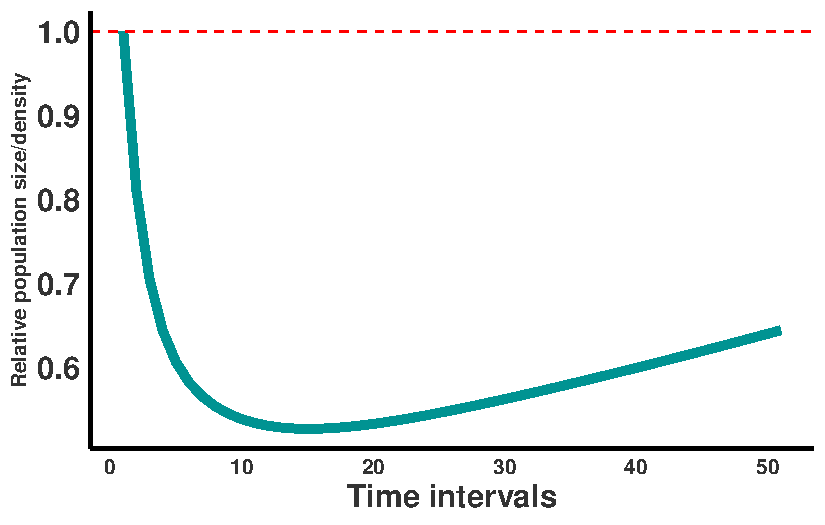
\includegraphics{112-Dinamica_de_Transiciones_files/figure-pdf/trans4-1.pdf}

\begin{Shaded}
\begin{Highlighting}[]
\CommentTok{\#plot(pr1, log = "y", ylim = c(0.1, 1.6), ann = FALSE)}
\CommentTok{\#title(main = "Proyección de la dinámica (Escenario 1)", xlab = "Time intervals", ylab = "Population size/density")}
\end{Highlighting}
\end{Shaded}

\begin{center}\rule{0.5\linewidth}{0.5pt}\end{center}

\subsubsection{Segundo escenario:}\label{segundo-escenario}

En este escenario, se supone que la población tiene una mayor proporción
de individuos en las categorías juvenil y adulto no reproductivo (0.15,
0.35, 0.30, 0.20). En este caso, la población decrece rápidamente en los
primeros periodos pero y despues de unos 5 periodos de tiempo la
poblacion comienza a crecer y tiene un tamaño población relativo al
comienzo despues de ±16 periodos de tiempo. Esto indica que la población
se recupera rápidamente y alcanza un tamaño poblacional estable en un
periodo relativamente corto.

\begin{center}\rule{0.5\linewidth}{0.5pt}\end{center}

\subsubsection{Tercer escenario (estructura
estable):}\label{tercer-escenario-estructura-estable}

Como la población tiene una estructura estable, la población no tiene un
crecimiento diferente a 1, por lo que alcanza un tamaño poblacional
estable en un periodo relativamente corto o inmediato. Debido que la
población tiene una estructura estable, el tamaño relativo de la
población es constante.

\begin{Shaded}
\begin{Highlighting}[]
\CommentTok{\#Escenario 3. Estructura estable}
\CommentTok{\# Estructura estable de estados}
\NormalTok{Wmax }\OtherTok{\textless{}{-}} \FunctionTok{stable.stage}\NormalTok{(Lr1)}
\NormalTok{nLr3 }\OtherTok{\textless{}{-}}\NormalTok{ Wmax}
\CommentTok{\#Gráfica de barras del escenario 3}
\CommentTok{\#barplot(nLr3, names.arg = 1:4)}
\CommentTok{\#title( main = "Escenario 3", xlab = "Categoría", ylab = "Proporción")}
\CommentTok{\#Proyección de la dinámica escenario 3}
\NormalTok{Lr1st }\OtherTok{\textless{}{-}}\NormalTok{ (Lr1 }\SpecialCharTok{/}\NormalTok{ lambda)}
\CommentTok{\#Lr1st}
\CommentTok{\#eigen(Lr1st)}
\NormalTok{pr3 }\OtherTok{\textless{}{-}} \FunctionTok{project}\NormalTok{(Lr1st, }\AttributeTok{vector =}\NormalTok{ Wmax, }\AttributeTok{time =} \DecValTok{50}\NormalTok{)}
\NormalTok{pr3df }\OtherTok{\textless{}{-}} \FunctionTok{as.data.frame}\NormalTok{(pr3)}
\NormalTok{pr3df}\SpecialCharTok{$}\NormalTok{time }\OtherTok{\textless{}{-}} \FunctionTok{seq}\NormalTok{(}\DecValTok{1}\NormalTok{, }\FunctionTok{nrow}\NormalTok{(pr3df), }\DecValTok{1}\NormalTok{)}
\FunctionTok{ggplot}\NormalTok{(pr3df, }\FunctionTok{aes}\NormalTok{(time, pr3)) }\SpecialCharTok{+}
  \FunctionTok{geom\_line}\NormalTok{(}\FunctionTok{aes}\NormalTok{(}\AttributeTok{color =} \StringTok{"blue"}\NormalTok{), }\AttributeTok{size =} \DecValTok{2}\NormalTok{) }\SpecialCharTok{+}
  \FunctionTok{geom\_hline}\NormalTok{(}\AttributeTok{yintercept =} \DecValTok{1}\NormalTok{, }\AttributeTok{linetype =} \StringTok{"dashed"}\NormalTok{, }\AttributeTok{color =} \StringTok{"red"}\NormalTok{) }\SpecialCharTok{+}
  \FunctionTok{xlab}\NormalTok{(}\StringTok{"Time intervals"}\NormalTok{) }\SpecialCharTok{+}
  \FunctionTok{ylab}\NormalTok{(}\StringTok{"Relative population size/density"}\NormalTok{) }\SpecialCharTok{+}
  \FunctionTok{theme\_minimal}\NormalTok{() }\SpecialCharTok{+}
  \FunctionTok{rlt\_style\_colour}\NormalTok{()}
\end{Highlighting}
\end{Shaded}

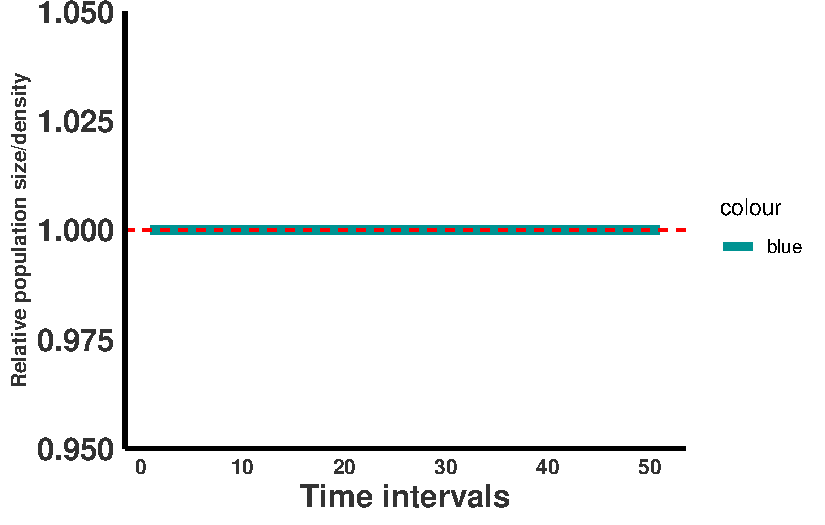
\includegraphics{112-Dinamica_de_Transiciones_files/figure-pdf/trans6-1.pdf}

\begin{Shaded}
\begin{Highlighting}[]
\DocumentationTok{\#\# Código para el plot usando el método tradicional}

\CommentTok{\#plot(pr3, log = "y", ylim = c(0.1, 1.6), ann = FALSE)}
\CommentTok{\#title(main = "Proyección de la dinámica (Escenario 3)", xlab = "Time intervals", ylab = "Population size/density")}
\end{Highlighting}
\end{Shaded}

\begin{center}\rule{0.5\linewidth}{0.5pt}\end{center}

\subsubsection{Cuarto escenario:}\label{cuarto-escenario}

En este escenario, se supone que la población tiene una mayor proporción
de plántulas y una proporción similar en las categorías juvenil, adulto
no reproductivo y adulto reproductivo (0.4, 0.2, 0.2, 0.2). En este
caso, la población decrece rápidamente en los primeros periodos pero y
después de unos ±7 periodos de tiempo la población comienza a crecer y
tiene un tamaño población relativo al comienzo después de ±36 periodos
de tiempo. Esto indica que la población se recupera rápidamente y
alcanza un tamaño poblacional estable en un periodo relativamente corto,
si la población comienza con esta estructura demográfica.

\begin{Shaded}
\begin{Highlighting}[]
\CommentTok{\# DINÁMICA POBLACIONAL ABSOLUTA.}

\NormalTok{nLr4 }\OtherTok{\textless{}{-}} \FunctionTok{c}\NormalTok{(}\DecValTok{66}\NormalTok{, }\DecValTok{33}\NormalTok{, }\DecValTok{33}\NormalTok{, }\DecValTok{33}\NormalTok{)}
\NormalTok{nLr4 }\OtherTok{\textless{}{-}}\NormalTok{ nLr4 }\SpecialCharTok{/} \FunctionTok{sum}\NormalTok{(nLr4)}

\NormalTok{pr4 }\OtherTok{\textless{}{-}} \FunctionTok{project}\NormalTok{(Lr1, }\AttributeTok{vector =}\NormalTok{ nLr4, }\AttributeTok{time =} \DecValTok{50}\NormalTok{)}
\NormalTok{pr4df }\OtherTok{\textless{}{-}} \FunctionTok{as.data.frame}\NormalTok{(pr4)}
\NormalTok{pr4df}\SpecialCharTok{$}\NormalTok{time }\OtherTok{\textless{}{-}} \FunctionTok{seq}\NormalTok{(}\DecValTok{1}\NormalTok{, }\FunctionTok{nrow}\NormalTok{(pr4df), }\DecValTok{1}\NormalTok{)}
\end{Highlighting}
\end{Shaded}

\begin{center}\rule{0.5\linewidth}{0.5pt}\end{center}

\subsubsection{Quinto escenario:}\label{quinto-escenario}

En este escenario, se supone que la población tiene una mayor proporción
de individuos en la categoría de adulto reproductivo (0,0,0,1). En el
escenario 5, la población crece rápidamente en los primeros periodos,
sufriendo una reducción después de ±5 meses; no obstante, se reconoce
que la población aumenta rápidamente.

\begin{Shaded}
\begin{Highlighting}[]
\CommentTok{\#Escenario 5. Límite superior}
\NormalTok{nLr5 }\OtherTok{\textless{}{-}} \FunctionTok{c}\NormalTok{(}\DecValTok{0}\NormalTok{, }\DecValTok{0}\NormalTok{, }\DecValTok{0}\NormalTok{, }\DecValTok{166}\NormalTok{)}
\CommentTok{\#Proporción de individuos por categoría}
\NormalTok{nLr5 }\OtherTok{\textless{}{-}}\NormalTok{ nLr5 }\SpecialCharTok{/} \FunctionTok{sum}\NormalTok{(nLr5)}
\CommentTok{\#nLr5}
\CommentTok{\#Gráfica de barras del escenario 5}
\CommentTok{\#barplot(nLr5, names.arg = 1:4)}
\CommentTok{\#title( main = "Escenario 5", xlab = "Categoría", ylab = "Proporción")}
\CommentTok{\#Proyección de la dinámica escenario 5}
\NormalTok{pr5 }\OtherTok{\textless{}{-}} \FunctionTok{project}\NormalTok{(Lr1, }\AttributeTok{vector =}\NormalTok{ nLr5, }\AttributeTok{time =} \DecValTok{50}\NormalTok{)}
\NormalTok{pr5df }\OtherTok{\textless{}{-}} \FunctionTok{as.data.frame}\NormalTok{(pr5)}
\NormalTok{pr5df}\SpecialCharTok{$}\NormalTok{time }\OtherTok{\textless{}{-}} \FunctionTok{seq}\NormalTok{(}\DecValTok{1}\NormalTok{, }\FunctionTok{nrow}\NormalTok{(pr5df), }\DecValTok{1}\NormalTok{)}
\FunctionTok{ggplot}\NormalTok{(pr5df, }\FunctionTok{aes}\NormalTok{(time, pr5)) }\SpecialCharTok{+}
  \FunctionTok{geom\_line}\NormalTok{(}\FunctionTok{aes}\NormalTok{(}\AttributeTok{color =} \StringTok{"blue"}\NormalTok{), }\AttributeTok{size =} \DecValTok{2}\NormalTok{) }\SpecialCharTok{+}
  \FunctionTok{geom\_hline}\NormalTok{(}\AttributeTok{yintercept =} \DecValTok{1}\NormalTok{, }\AttributeTok{linetype =} \StringTok{"dashed"}\NormalTok{, }\AttributeTok{color =} \StringTok{"red"}\NormalTok{) }\SpecialCharTok{+}
  \FunctionTok{xlab}\NormalTok{(}\StringTok{"Time intervals"}\NormalTok{) }\SpecialCharTok{+}
  \FunctionTok{ylab}\NormalTok{(}\StringTok{"Relative population size/density"}\NormalTok{) }\SpecialCharTok{+}
  \FunctionTok{theme\_minimal}\NormalTok{() }\SpecialCharTok{+}
  \FunctionTok{rlt\_style\_colour}\NormalTok{()}
\end{Highlighting}
\end{Shaded}

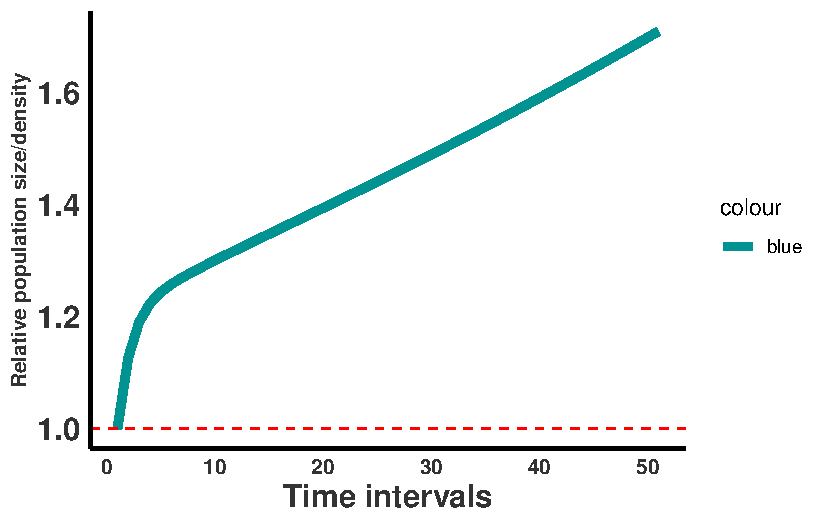
\includegraphics{112-Dinamica_de_Transiciones_files/figure-pdf/trans8-1.pdf}

\begin{Shaded}
\begin{Highlighting}[]
\CommentTok{\#plot(pr5, log = "y", ylim = c(0.1, 1.6), ann = FALSE)}
\CommentTok{\#title(main = "Proyección de la dinámica (Escenario 5)", xlab = "Time intervals", ylab = "Population size/density")}
\end{Highlighting}
\end{Shaded}

\begin{center}\rule{0.5\linewidth}{0.5pt}\end{center}

\subsection{Gráfica de la dinámica
absoluta}\label{gruxe1fica-de-la-dinuxe1mica-absoluta}

En el siguiente recuadro se integran en una sola gráfica los resultados
de la dinámica absoluta de \emph{L. rubripetala} para los escenarios 1,
3 y 5.

`

\begin{center}\rule{0.5\linewidth}{0.5pt}\end{center}

\subsection{Gráfica de la dinámica
absoluta}\label{gruxe1fica-de-la-dinuxe1mica-absoluta-1}

\begin{Shaded}
\begin{Highlighting}[]
\FunctionTok{ggplot}\NormalTok{(Population\_density, }\FunctionTok{aes}\NormalTok{(time, Pop, }\AttributeTok{color =}\NormalTok{ Escenario)) }\SpecialCharTok{+}
  \FunctionTok{geom\_line}\NormalTok{(}\AttributeTok{size =} \DecValTok{1}\NormalTok{) }\SpecialCharTok{+}
  \FunctionTok{geom\_hline}\NormalTok{(}\AttributeTok{yintercept =} \DecValTok{1}\NormalTok{, }\AttributeTok{linetype =} \StringTok{"dashed"}\NormalTok{, }\AttributeTok{color =} \StringTok{"red"}\NormalTok{) }\SpecialCharTok{+}
  \FunctionTok{labs}\NormalTok{(}
    \AttributeTok{title =} \StringTok{"Population dynamics projections"}\NormalTok{,}
    \AttributeTok{x =} \StringTok{"Time intervals"}\NormalTok{,}
    \AttributeTok{y =} \StringTok{"Relative population size/density"}
\NormalTok{  ) }\SpecialCharTok{+}
  \FunctionTok{theme\_minimal}\NormalTok{() }\SpecialCharTok{+}
  \FunctionTok{rlt\_style\_colour}\NormalTok{()}
\end{Highlighting}
\end{Shaded}

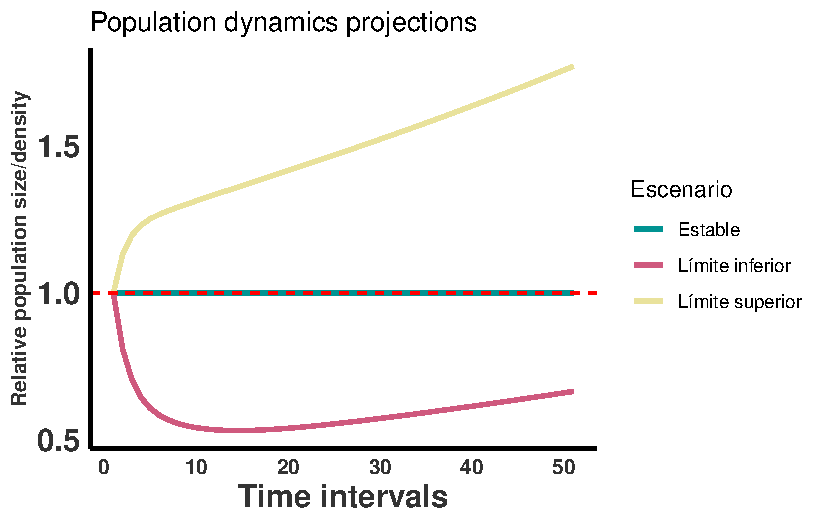
\includegraphics{112-Dinamica_de_Transiciones_files/figure-pdf/trans10-1.pdf}

\begin{center}\rule{0.5\linewidth}{0.5pt}\end{center}

\begin{center}\rule{0.5\linewidth}{0.5pt}\end{center}

\section{Dinámica poblacional transitoria
estandarizada}\label{dinuxe1mica-poblacional-transitoria-estandarizada}

La dinámica poblacional transitoria estandarizada proyecta de forma
cuantitativa los cambios en la población a corto plazo para los
escenarios planteados. Con este fin, primero se elimina el efecto de
largo plazo de la tasa de crecimiento poblacional y de la estructura
inicial de la población, lo cual permite mantener otras propiedades
asintóticas, por ejemplo, la estructura estable de estados/edades y las
elasticidades (Koons, Iles \& Stott, 2021). En este proceso se dividen
todos los elementos de la matriz sobre el valor de la lambda asintótica
(\(λ_{max}\)) obtenida por la iteración de la matriz y se escala a 1 el
vector de la estructura poblacional (Koons, Iles \& Stott, 2021). Como
resultado de este proceso, y para cualquier matriz y vector
estandarizados, tendremos una \(λ_{max}\) igual a la unidad y la suma de
1 en el segundo caso, lo cual facilita y hace equitativa la comparación
entre los modelos de los distintos escenarios (Stott, Townley \&
Hodgson, 2011; Stott, Hodgson \& Townley, 2012b; Stott, Hodgson \&
Townley, 2012a; Koons, Iles \& Stott, 2021).

En el árticulo de Tremblay y colaboradores (Tremblay, Raventos \&
Ackerman, 2015), la dinámica transitoria para \emph{L. reubripetala}
corresponde a la figura 2B. Esta figura se construye con base en la
matriz y vectores estandarizados de los cinco escenarios definidos y se
proyecta el crecimiento de la población a 50 meses (4.1 años). Las
gráficas de la dinámica transitoria para estos escenarios se generan
usando las siguientes funciones de \emph{R}: \emph{standard.A=T} en la
estandarización de la matriz y \emph{standard.vec=T} para el vector,
\emph{project} para la estimar la tendencia del crecimiento poblacional
(Stott, Townley \& Hodgson, 2011; Stott, Hodgson \& Townley, 2012b;
Stott, Hodgson \& Townley, 2012a) y \emph{ggplot} (Programa de \emph{R})
para agrupar en una sola gráfica la tendencia del crecimiento
poblacional de los escenarios.

En el siguiente recuadro se estima el crecimiento poblacional de
\emph{L. rubripetala} sin efecto de la dinámica asintótica para tres
escenarios: 1, 3 y 5. En el cálculo de la dinámica de corto plazo se
proyecta se usa la matriz de transición de la población 1 de \emph{L.
reubripetala} y el correspondiente vector inicial de la población.

\begin{Shaded}
\begin{Highlighting}[]
\DocumentationTok{\#\# PROYECCIÓN DE LA DINÁMICA DE CORTO PLAZO. }

\CommentTok{\#Vector de estructura inicial: abundancia por categoría de acuerdo con  el estado}
\NormalTok{n0 }\OtherTok{\textless{}{-}} \FunctionTok{c}\NormalTok{(}\DecValTok{166}\NormalTok{, }\DecValTok{0}\NormalTok{, }\DecValTok{0}\NormalTok{, }\DecValTok{0}\NormalTok{)}

\CommentTok{\#Escenario 1: Límite inferior}
\NormalTok{pr2}\FloatTok{.1} \OtherTok{\textless{}{-}} \FunctionTok{project}\NormalTok{(}
\NormalTok{  Lr1,}
  \AttributeTok{vector =}\NormalTok{ nLr1,}
  \AttributeTok{time =} \DecValTok{50}\NormalTok{,}
  \AttributeTok{standard.A =}\NormalTok{ T,}
  \AttributeTok{standard.vec =}\NormalTok{ T}
\NormalTok{)}

\CommentTok{\#Escenario 3. Estructura estable}
\NormalTok{pr2}\FloatTok{.3} \OtherTok{\textless{}{-}} \FunctionTok{project}\NormalTok{(}
\NormalTok{  Lr1,}
  \AttributeTok{vector =}\NormalTok{ nLr3,}
  \AttributeTok{time =} \DecValTok{50}\NormalTok{,}
  \AttributeTok{standard.A =}\NormalTok{ T,}
  \AttributeTok{standard.vec =}\NormalTok{ T}
\NormalTok{)}

\CommentTok{\#Escenario 5. Límite superior}
\NormalTok{pr2}\FloatTok{.5} \OtherTok{\textless{}{-}} \FunctionTok{project}\NormalTok{(}
\NormalTok{  Lr1,}
  \AttributeTok{vector =}\NormalTok{ nLr5,}
  \AttributeTok{time =} \DecValTok{50}\NormalTok{,}
  \AttributeTok{standard.A =}\NormalTok{ T,}
  \AttributeTok{standard.vec =}\NormalTok{ T}
\NormalTok{)}
\end{Highlighting}
\end{Shaded}

\begin{center}\rule{0.5\linewidth}{0.5pt}\end{center}

\section{Gráfica de la dinámica poblacional transitoria estandarizada
por
escenario}\label{gruxe1fica-de-la-dinuxe1mica-poblacional-transitoria-estandarizada-por-escenario}

La proyección de la dinámica transitoria para los tres escenarios
definidos (1, 3, y 5) tiene un comportamiento contrastante, lo cual es
evidente en la gráfica del siguiente recuadro. El crecimiento es
constante (i.e.~lambda =1) cuando se considera la estructura estable de
estados. Cuando la estructura poblacional corresponde al Inicio I se
determina un decremento en la población en los primeros 5 meses, el cual
se mantiene en el tiempo a lo largo de la proyección. Si la población
está representada por adultos reproductivos, ésta crece en los primeros
cinco meses y este crecimiento se mantiene a lo largo de los 50 meses.

\begin{Shaded}
\begin{Highlighting}[]
\CommentTok{\# DINÁMICA POBLACIONAL TRANSITORIA ESTANDARIZADA {-}{-}{-}{-}{-}{-}{-}{-}{-}{-} \#}
\CommentTok{\# Gráfica de la Dinámica transitoria específica de la población  }

\FunctionTok{layout}\NormalTok{(}\FunctionTok{matrix}\NormalTok{(}\FunctionTok{c}\NormalTok{(}\DecValTok{1}\NormalTok{, }\DecValTok{2}\NormalTok{, }\DecValTok{3}\NormalTok{), }\AttributeTok{ncol =} \DecValTok{3}\NormalTok{))}
\CommentTok{\#par(mfrow=c(3,1))}

\CommentTok{\# Gráfica dinámica corto plazo: Inicio I}
\FunctionTok{plot}\NormalTok{(}
\NormalTok{  pr2}\FloatTok{.2}\NormalTok{,}
  \AttributeTok{log =} \StringTok{"y"}\NormalTok{,}
  \AttributeTok{main =} \StringTok{"Escenario 2"}\NormalTok{,}
  \AttributeTok{xlab =} \StringTok{""}\NormalTok{,}
  \AttributeTok{ylab =} \StringTok{"Densidad poblacional"}
\NormalTok{)}

\CommentTok{\# Gráfica dinámica corto plazo: Estructura Estable}
\FunctionTok{plot}\NormalTok{(pr2}\FloatTok{.3}\NormalTok{, }\AttributeTok{log =} \StringTok{"y"}\NormalTok{, }\AttributeTok{main =} \StringTok{"Escenario 3"}\NormalTok{, }\AttributeTok{xlab =} \StringTok{""}\NormalTok{, }\AttributeTok{ylab =} \StringTok{""}\NormalTok{)}
\end{Highlighting}
\end{Shaded}

\begin{verbatim}
Warning in plot.window(...): axis(2, *): range of values ( 0) is small wrt |M|
= 1 --> not pretty()
\end{verbatim}

\begin{Shaded}
\begin{Highlighting}[]
\CommentTok{\# Gráfica dinámica corto plazo: Límite superior}
\FunctionTok{plot}\NormalTok{(pr2}\FloatTok{.5}\NormalTok{, }\AttributeTok{log =} \StringTok{"y"}\NormalTok{, }\AttributeTok{main =} \StringTok{"Escenario 5"}\NormalTok{, }\AttributeTok{xlab =} \StringTok{""}\NormalTok{, }\AttributeTok{ylab =} \StringTok{""}\NormalTok{)}
\end{Highlighting}
\end{Shaded}

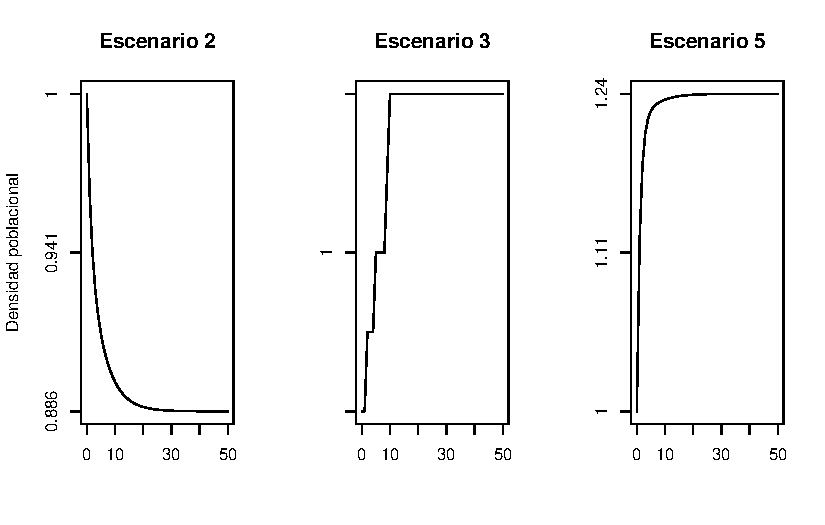
\includegraphics{112-Dinamica_de_Transiciones_files/figure-pdf/trans14-1.pdf}

\begin{center}\rule{0.5\linewidth}{0.5pt}\end{center}

\section{Gráfica de la dinámica poblacional transitoria
estandarizada}\label{gruxe1fica-de-la-dinuxe1mica-poblacional-transitoria-estandarizada}

En el siguiente recuadro se integran en una sola gráfica los resultados
de la dinámica poblacional transitoria estandarizada de \emph{L.
rubripetala} para los escenarios 1, 3 y 5.

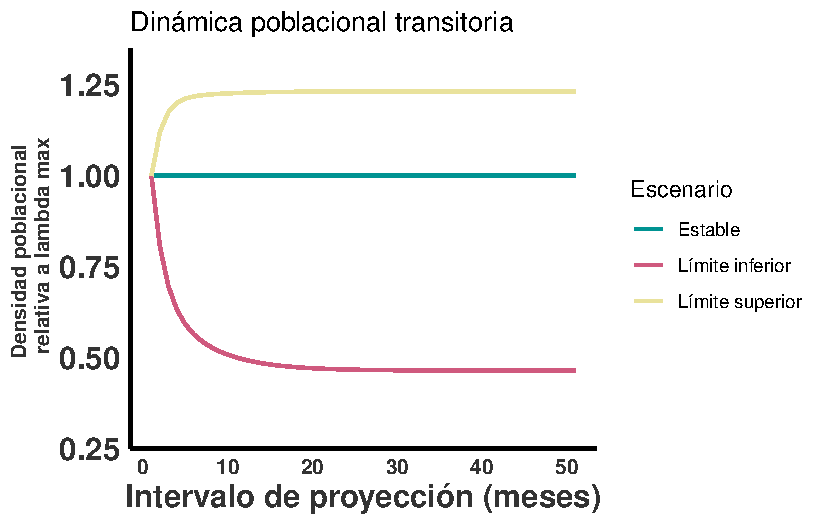
\includegraphics{112-Dinamica_de_Transiciones_files/figure-pdf/trans15-1.pdf}

La gráfica a continuación corresponde a los cinco escenarios planteados
para la población 1 de \emph{L. rubripetala}, semejante a la figura 2B
del artículo de Tremblay y colaboradores (Tremblay, Raventos \&
Ackerman, 2015); aunque cabe señalar que no se integran los índices
transitorios, los cuales abordamos a continuación.

\begin{center}\rule{0.5\linewidth}{0.5pt}\end{center}

\subsection{Índices de transitorios.}\label{uxedndices-de-transitorios.}

Se determinan los \emph{límites de la dinámica transitoria} con el fin
de evaluar en el corto plazo los cambios cuantitativos en la población,
debido a perturbaciones repentinas en la estructura poblacional. Estos
se calculan en los modelos de corto plazo a través de los \emph{Índices
de transferencia} (Stott, Townley \& Hodgson, 2011), los cuales se
estiman previo a que se alcance la tasa constante de crecimiento
poblacional e incluyen los siguiente tres parámetros:

\emph{i}) \emph{Reactividad alta y Reactividad baja} (Upper reactivity y
Lower reactivity) que representan el crecimiento o el decremento
inmediato (i.e.~primer intervalo de tiempo).

\emph{ii}) \emph{Máxima amplificación y Máxima atenuación} (Maximum
amplification y Maximum attenuation) que indican, respectivamente, el
incremento o decremento máximo futuro del crecimiento poblacional.

\emph{iii}) \emph{Inercia alta e Inercia baja} (Upper inertia y Lower
inertia) que evalúan el límite más alto o el más bajo en el crecimiento
de la población.

\subsubsection{Cálculo de los límites
transitorios}\label{cuxe1lculo-de-los-luxedmites-transitorios}

\begin{itemize}
\tightlist
\item
  Escenario 1 (límite inferior):
\end{itemize}

\begin{Shaded}
\begin{Highlighting}[]
\CommentTok{\#Escenario 1 (límite inferior):}
\NormalTok{lim.trans }\OtherTok{\textless{}{-}} \FunctionTok{as.data.frame}\NormalTok{(}\FunctionTok{matrix}\NormalTok{(}\ConstantTok{NA}\NormalTok{, }\DecValTok{5}\NormalTok{, }\DecValTok{3}\NormalTok{))}
\FunctionTok{names}\NormalTok{(lim.trans) }\OtherTok{\textless{}{-}} \FunctionTok{c}\NormalTok{(}\StringTok{"reac"}\NormalTok{, }\StringTok{"maxatt"}\NormalTok{, }\StringTok{"inertia"}\NormalTok{)}

\NormalTok{reac1 }\OtherTok{\textless{}{-}} \FunctionTok{reac}\NormalTok{(Lr1, }\AttributeTok{vector =}\NormalTok{ nLr1)}
\NormalTok{lim.trans[}\DecValTok{1}\NormalTok{, }\DecValTok{1}\NormalTok{] }\OtherTok{\textless{}{-}}\NormalTok{ reac1}
\NormalTok{reac1}
\end{Highlighting}
\end{Shaded}

\begin{verbatim}
[1] 0.8049991
\end{verbatim}

\begin{Shaded}
\begin{Highlighting}[]
\NormalTok{maxatt1 }\OtherTok{\textless{}{-}} \FunctionTok{maxatt}\NormalTok{(Lr1, }\AttributeTok{vector =}\NormalTok{ nLr1, }\AttributeTok{return.t =}\NormalTok{ T)}
\NormalTok{maxatt1}
\end{Highlighting}
\end{Shaded}

\begin{verbatim}
$maxatt
[1] 0.4643848

$t
[1] 49
\end{verbatim}

\begin{Shaded}
\begin{Highlighting}[]
\NormalTok{lim.trans[}\DecValTok{1}\NormalTok{, }\DecValTok{2}\NormalTok{] }\OtherTok{\textless{}{-}}\NormalTok{ maxatt1[}\DecValTok{1}\NormalTok{]}

\NormalTok{inertia1 }\OtherTok{\textless{}{-}} \FunctionTok{inertia}\NormalTok{(Lr1, }\AttributeTok{vector =}\NormalTok{ nLr1)}
\NormalTok{inertia1}
\end{Highlighting}
\end{Shaded}

\begin{verbatim}
[1] 0.4643642
\end{verbatim}

\begin{Shaded}
\begin{Highlighting}[]
\NormalTok{lim.trans[}\DecValTok{1}\NormalTok{, }\DecValTok{3}\NormalTok{] }\OtherTok{\textless{}{-}}\NormalTok{ inertia1}
\end{Highlighting}
\end{Shaded}

\begin{center}\rule{0.5\linewidth}{0.5pt}\end{center}

\begin{itemize}
\tightlist
\item
  Escenario 3 (estructura estable):
\end{itemize}

\begin{Shaded}
\begin{Highlighting}[]
\CommentTok{\#Escenario 3 (estructura estable):}
\NormalTok{reac3 }\OtherTok{\textless{}{-}} \FunctionTok{reac}\NormalTok{(Lr1, }\AttributeTok{vector =}\NormalTok{ nLr3)}
\NormalTok{lim.trans[}\DecValTok{3}\NormalTok{, }\DecValTok{1}\NormalTok{] }\OtherTok{\textless{}{-}}\NormalTok{ reac3}
\NormalTok{reac3}
\end{Highlighting}
\end{Shaded}

\begin{verbatim}
[1] 1
\end{verbatim}

\begin{Shaded}
\begin{Highlighting}[]
\NormalTok{inertia3 }\OtherTok{\textless{}{-}} \FunctionTok{inertia}\NormalTok{(Lr1, }\AttributeTok{vector =}\NormalTok{ nLr3)}
\NormalTok{inertia3}
\end{Highlighting}
\end{Shaded}

\begin{verbatim}
[1] 1
\end{verbatim}

\begin{Shaded}
\begin{Highlighting}[]
\NormalTok{lim.trans[}\DecValTok{3}\NormalTok{, }\DecValTok{3}\NormalTok{] }\OtherTok{\textless{}{-}}\NormalTok{ inertia3}
\end{Highlighting}
\end{Shaded}

\begin{center}\rule{0.5\linewidth}{0.5pt}\end{center}

\begin{itemize}
\tightlist
\item
  Escenario 5 (límite superior):
\end{itemize}

\begin{Shaded}
\begin{Highlighting}[]
\CommentTok{\#Escenario 5. Límite superior}
\NormalTok{reac5 }\OtherTok{\textless{}{-}} \FunctionTok{reac}\NormalTok{(Lr1, }\AttributeTok{vector =}\NormalTok{ nLr5)}
\NormalTok{lim.trans[}\DecValTok{5}\NormalTok{, }\DecValTok{1}\NormalTok{] }\OtherTok{\textless{}{-}}\NormalTok{ reac5}
\NormalTok{reac5}
\end{Highlighting}
\end{Shaded}

\begin{verbatim}
[1] 1.122908
\end{verbatim}

\begin{Shaded}
\begin{Highlighting}[]
\NormalTok{maxamp5 }\OtherTok{\textless{}{-}} \FunctionTok{maxamp}\NormalTok{(Lr1, }\AttributeTok{vector =}\NormalTok{ nLr5, }\AttributeTok{return.t =}\NormalTok{ T, }\AttributeTok{conv.accuracy =} \FloatTok{0.01}\NormalTok{)}
\NormalTok{maxamp5}
\end{Highlighting}
\end{Shaded}

\begin{verbatim}
$maxamp
[1] 1.223337

$t
[1] 5
\end{verbatim}

\begin{Shaded}
\begin{Highlighting}[]
\NormalTok{lim.trans[}\DecValTok{5}\NormalTok{, }\DecValTok{2}\NormalTok{] }\OtherTok{\textless{}{-}}\NormalTok{ maxamp5[}\DecValTok{1}\NormalTok{]}
\NormalTok{inertia5 }\OtherTok{\textless{}{-}} \FunctionTok{inertia}\NormalTok{(Lr1, }\AttributeTok{vector =}\NormalTok{ nLr5)}
\NormalTok{inertia5}
\end{Highlighting}
\end{Shaded}

\begin{verbatim}
[1] 1.23738
\end{verbatim}

\begin{Shaded}
\begin{Highlighting}[]
\NormalTok{lim.trans[}\DecValTok{5}\NormalTok{, }\DecValTok{3}\NormalTok{] }\OtherTok{\textless{}{-}}\NormalTok{ inertia5}
\end{Highlighting}
\end{Shaded}

\subsubsection{Crear una tabla de los indices
transitorios}\label{crear-una-tabla-de-los-indices-transitorios}

\begin{Shaded}
\begin{Highlighting}[]
\CommentTok{\#Escenario 2 (inicio I):}
\NormalTok{reac2 }\OtherTok{\textless{}{-}} \FunctionTok{reac}\NormalTok{(Lr1, }\AttributeTok{vector =}\NormalTok{ nLr2)}
\NormalTok{reac2}
\NormalTok{lim.trans[}\DecValTok{2}\NormalTok{, }\DecValTok{1}\NormalTok{] }\OtherTok{\textless{}{-}}\NormalTok{ reac2}
\NormalTok{maxatt2 }\OtherTok{\textless{}{-}} \FunctionTok{maxatt}\NormalTok{(Lr1, }\AttributeTok{vector =}\NormalTok{ nLr2, }\AttributeTok{return.t =}\NormalTok{ T)}
\NormalTok{maxatt2}
\NormalTok{lim.trans[}\DecValTok{2}\NormalTok{, }\DecValTok{2}\NormalTok{] }\OtherTok{\textless{}{-}}\NormalTok{ maxatt2[}\DecValTok{1}\NormalTok{]}
\NormalTok{inertia2 }\OtherTok{\textless{}{-}} \FunctionTok{inertia}\NormalTok{(Lr1, }\AttributeTok{vector =}\NormalTok{ nLr2)}
\NormalTok{inertia2}
\NormalTok{lim.trans[}\DecValTok{2}\NormalTok{, }\DecValTok{3}\NormalTok{] }\OtherTok{\textless{}{-}}\NormalTok{ inertia2}

\CommentTok{\#Escenario 4. Inicio II}
\NormalTok{reac4 }\OtherTok{\textless{}{-}} \FunctionTok{reac}\NormalTok{(Lr1, }\AttributeTok{vector =}\NormalTok{ nLr4)}
\NormalTok{lim.trans[}\DecValTok{4}\NormalTok{, }\DecValTok{1}\NormalTok{] }\OtherTok{\textless{}{-}}\NormalTok{ reac4}
\NormalTok{reac4}
\NormalTok{maxatt4 }\OtherTok{\textless{}{-}} \FunctionTok{maxatt}\NormalTok{(Lr1, }\AttributeTok{vector =}\NormalTok{ nLr4, }\AttributeTok{return.t =}\NormalTok{ T)}
\NormalTok{maxatt4}
\NormalTok{lim.trans[}\DecValTok{4}\NormalTok{, }\DecValTok{2}\NormalTok{] }\OtherTok{\textless{}{-}}\NormalTok{ maxatt4[}\DecValTok{1}\NormalTok{]}
\NormalTok{inertia4 }\OtherTok{\textless{}{-}} \FunctionTok{inertia}\NormalTok{(Lr1, }\AttributeTok{vector =}\NormalTok{ nLr4)}
\NormalTok{inertia4}
\NormalTok{lim.trans[}\DecValTok{4}\NormalTok{, }\DecValTok{3}\NormalTok{] }\OtherTok{\textless{}{-}}\NormalTok{ inertia4}
\end{Highlighting}
\end{Shaded}

\begin{center}\rule{0.5\linewidth}{0.5pt}\end{center}

\subsection{Tabla de los indices
transitorios}\label{tabla-de-los-indices-transitorios}

En la tabla del siguiente recuadro se resumen los valores estimados por
escenario.

\begin{Shaded}
\begin{Highlighting}[]
\FunctionTok{gt}\NormalTok{(lim.trans)}
\end{Highlighting}
\end{Shaded}

\begin{table}
\fontsize{12.0pt}{14.0pt}\selectfont
\begin{tabular*}{\linewidth}{@{\extracolsep{\fill}}rrr}
\toprule
reac & maxatt & inertia \\ 
\midrule\addlinespace[2.5pt]
0.8049991 & 0.4643848 & 0.4643642 \\ 
0.9628771 & 0.8863718 & 0.8863327 \\ 
1.0000000 & NA & 1.0000000 \\ 
0.9273971 & 0.7894384 & 0.7894036 \\ 
1.1229083 & 1.2233368 & 1.2373800 \\ 
\bottomrule
\end{tabular*}
\end{table}

\begin{center}\rule{0.5\linewidth}{0.5pt}\end{center}

\section{Gráfica de dinámica poblacional transitoria, integrando los
índices transitorios: escenarios 1, 3 y
5.}\label{gruxe1fica-de-dinuxe1mica-poblacional-transitoria-integrando-los-uxedndices-transitorios-escenarios-1-3-y-5.}

En el siguiente recuadro se integran en una sola gráfica los resultados
de la dinámica transitoria estandarizada de \emph{L. rubripetala} para
los escenarios 1, 3 y 5.

\begin{Shaded}
\begin{Highlighting}[]
\NormalTok{len }\OtherTok{\textless{}{-}} \FunctionTok{nrow}\NormalTok{(pr2}\FloatTok{.1}\NormalTok{)}
\NormalTok{Population\_density }\OtherTok{\textless{}{-}} \FunctionTok{rbind}\NormalTok{(}
  \FunctionTok{data.frame}\NormalTok{(}\AttributeTok{Projection =}\NormalTok{ pr2}\FloatTok{.1}\NormalTok{, }\AttributeTok{Escenario =} \StringTok{"Límite inferior"}\NormalTok{),}
  \FunctionTok{data.frame}\NormalTok{(}\AttributeTok{Projection =}\NormalTok{ pr2}\FloatTok{.3}\NormalTok{, }\AttributeTok{Escenario =} \StringTok{"Estable"}\NormalTok{),}
  \FunctionTok{data.frame}\NormalTok{(}\AttributeTok{Projection =}\NormalTok{ pr2}\FloatTok{.5}\NormalTok{, }\AttributeTok{Escenario =} \StringTok{"Límite superior"}\NormalTok{)}
\NormalTok{)}
\NormalTok{Population\_density}\SpecialCharTok{$}\NormalTok{Time }\OtherTok{\textless{}{-}} \FunctionTok{rep}\NormalTok{(}\FunctionTok{seq}\NormalTok{(}\DecValTok{1}\NormalTok{, len, }\DecValTok{1}\NormalTok{), }\DecValTok{3}\NormalTok{)}

\NormalTok{trans.plot }\OtherTok{\textless{}{-}} \FunctionTok{ggplot}\NormalTok{(}\AttributeTok{data =}\NormalTok{ Population\_density) }\SpecialCharTok{+}
  \FunctionTok{theme\_minimal}\NormalTok{() }\SpecialCharTok{+}
  \CommentTok{\# theme(panel.border = element\_blank()) +}
  \CommentTok{\#theme(legend.position = "none") +}
  \FunctionTok{geom\_line}\NormalTok{(}
    \FunctionTok{aes}\NormalTok{(}\AttributeTok{x =}\NormalTok{ Time, }\AttributeTok{y =}\NormalTok{ Projection, }\AttributeTok{group =}\NormalTok{ Escenario, }\AttributeTok{colour =}\NormalTok{ Escenario),}
    \AttributeTok{linewidth =} \FloatTok{0.8}
\NormalTok{  ) }\SpecialCharTok{+}
  \FunctionTok{scale\_colour\_manual}\NormalTok{(}\AttributeTok{values =} \FunctionTok{c}\NormalTok{(}\StringTok{"green4"}\NormalTok{, }\StringTok{"black"}\NormalTok{, }\StringTok{"orange2"}\NormalTok{)) }\SpecialCharTok{+}
  \FunctionTok{labs}\NormalTok{(}
    \AttributeTok{title =} \StringTok{"Dinámica poblacional transitoria"}\NormalTok{,}
    \AttributeTok{x =} \StringTok{"Intervalo de proyección (meses)"}\NormalTok{,}
    \AttributeTok{y =} \StringTok{"Densidad poblacional relativa }\SpecialCharTok{\textbackslash{}n}\StringTok{ a lambda max"}
\NormalTok{  ) }\SpecialCharTok{+}
  \FunctionTok{ylim}\NormalTok{(}\FloatTok{0.3}\NormalTok{, }\FloatTok{1.3}\NormalTok{) }\SpecialCharTok{+}
  \FunctionTok{rlt\_style\_colour}\NormalTok{()}


\NormalTok{trans.plot }\SpecialCharTok{+}
  \FunctionTok{annotate}\NormalTok{(}
    \StringTok{"text"}\NormalTok{,}
    \AttributeTok{x =} \DecValTok{49}\NormalTok{,}
    \AttributeTok{y =}\NormalTok{ maxatt1}\SpecialCharTok{$}\NormalTok{maxatt,}
    \CommentTok{\# 1. Change expression() to a string}
    \CommentTok{\# 2. Add parse = TRUE}
    \AttributeTok{label =} \StringTok{"underline(rho) == 0.46"}\NormalTok{,}
    \AttributeTok{parse =} \ConstantTok{TRUE}\NormalTok{,}
    \AttributeTok{hjust =} \FloatTok{1.0}\NormalTok{,}
    \AttributeTok{vjust =} \SpecialCharTok{{-}}\DecValTok{1}
\NormalTok{  ) }\SpecialCharTok{+}
  \FunctionTok{annotate}\NormalTok{(}
    \StringTok{"text"}\NormalTok{,}
    \AttributeTok{x =} \DecValTok{49}\NormalTok{,}
    \AttributeTok{y =}\NormalTok{ maxamp5}\SpecialCharTok{$}\NormalTok{maxamp,}
    \CommentTok{\# 1. Change expression() to a string}
    \CommentTok{\# 2. Add parse = TRUE}
    \AttributeTok{label =} \StringTok{"bar(rho) == 1"}\NormalTok{,}
    \AttributeTok{parse =} \ConstantTok{TRUE}\NormalTok{,}
    \AttributeTok{hjust =} \FloatTok{1.22}\NormalTok{,}
    \AttributeTok{vjust =} \SpecialCharTok{{-}}\DecValTok{1}
\NormalTok{  )}
\end{Highlighting}
\end{Shaded}

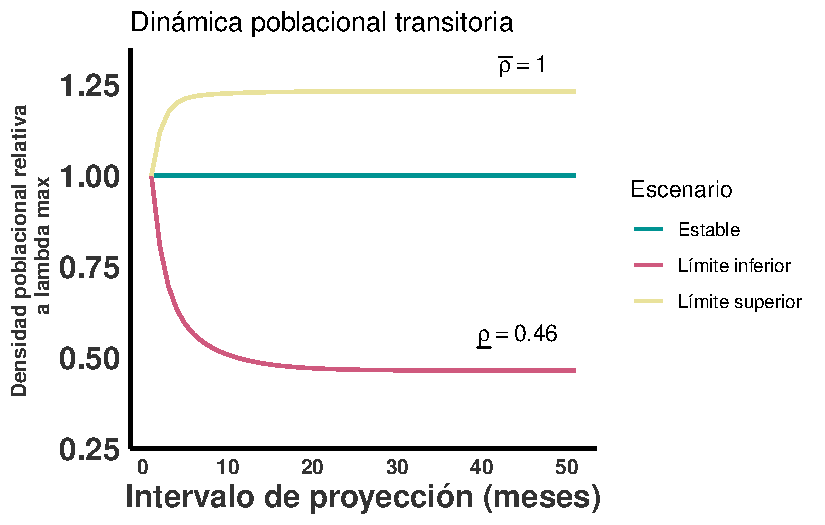
\includegraphics{112-Dinamica_de_Transiciones_files/figure-pdf/trans22-1.pdf}

\begin{center}\rule{0.5\linewidth}{0.5pt}\end{center}

La gráfica a continuación corresponde a los cinco escenarios planteados
para la población 1 de \emph{L. rubripetala}, equivalente a la figura 2B
del artículo de Tremblay y colaboradores ((Tremblay, Raventos \&
Ackerman, 2015)). Esta permitirá comparar tus resultados y verificar que
los escenarios que haz desarrollado estén correctos.

Revisión:

RLT: 2025\_06\_09

\phantomsection\label{refs}
\begin{CSLReferences}{1}{0}
\bibitem[\citeproctext]{ref-bierzychudek1999looking}
Bierzychudek P. 1999. Looking backwards: Assessing the projections of a
transition matrix model. \emph{Ecological Applications} 9:1278--1287.

\bibitem[\citeproctext]{ref-caswell2000matrix}
Caswell H. 1989. \emph{Matrix {P}opulation {M}odels}. Sinauer
Sunderland, MA.

\bibitem[\citeproctext]{ref-crone2011plant}
Crone EE, Menges ES, Ellis MM, Bell T, Bierzychudek P, Ehrlén J, Kaye
TN, Knight TM, Lesica P, Morris WF, others. 2011. How do plant
ecologists use matrix population models? \emph{Ecology Letters} 14:1--8.

\bibitem[\citeproctext]{ref-ezard2010matrix}
Ezard TH, Bullock JM, Dalgleish HJ, Millon A, Pelletier F, Ozgul A,
Koons DN. 2010. Matrix models for a changeable world: The importance of
transient dynamics in population management. \emph{Journal of Applied
Ecology} 47:515--523.

\bibitem[\citeproctext]{ref-hinrichsen2025solving}
Hinrichsen RA. 2025. Solving three core challenges in transient dynamics
analysis of matrix population models. \emph{bioRxiv}:2025--05.

\bibitem[\citeproctext]{ref-koons2021transient}
Koons DN, Iles DT, Stott I. 2021. Transient analyses of population
dynamics using matrix projection models. \emph{Demographic Methods
across the Tree of Life (Oxford University PressOxford, 2021)
p}:197--212.

\bibitem[\citeproctext]{ref-ospina2023effect}
Ospina-Calderón N, Tremblay R, Torres A, Flanagan N. 2023. The effect of
habitat transformation on a twig epiphytic orchid: Evidence from
population dynamics. \emph{Frontiers in Ecology and Evolution}
11:1135316.

\bibitem[\citeproctext]{ref-raventos2015transient}
Raventós J, González E, Mújica E, Bonet A. 2015. Transient population
dynamics of two epiphytic orchid species after {H}urricane {I}van:
Implications for management. \emph{Biotropica} 47:441--448. DOI:
\href{https://doi.org/10.1111/btp.12231}{10.1111/btp.12231}.

\bibitem[\citeproctext]{ref-schodelbauerova2010prediction}
Schödelbauerová I, Tremblay R, Kindlmann P. 2010. Prediction vs.
Reality: Can a PVA model predict population persistence 13 years later?
\emph{Biodiversity and Conservation} 19:637--650. DOI:
\href{https://doi.org/10.1007/s10531-009-9724-1}{10.1007/s10531-009-9724-1}.

\bibitem[\citeproctext]{ref-stott2012modelling}
Stott IM. 2012. \emph{Modelling transient population dynamics and their
role in ecology and evolution}. University of Exeter (United Kingdom).

\bibitem[\citeproctext]{ref-stott2010boom}
Stott I, Franco M, Carslake D, Townley S, Hodgson D. 2010. Boom or bust?
A comparative analysis of transient population dynamics in plants.
\emph{Journal of Ecology} 98:302--311.

\bibitem[\citeproctext]{ref-stott2012popdemo}
Stott I, Hodgson DJ, Townley S. 2012b. {p}opdemo: An {R} package for
population demography using projection matrix analysis. \emph{Methods in
Ecology and Evolution} 3:797--802.

\bibitem[\citeproctext]{ref-stott2012beyond}
Stott I, Hodgson DJ, Townley S. 2012a. Beyond sensitivity: Nonlinear
perturbation analysis of transient dynamics. \emph{Methods in Ecology
and Evolution} 3:673--684.

\bibitem[\citeproctext]{ref-stott2011framework}
Stott I, Townley S, Hodgson DJ. 2011. A framework for studying transient
dynamics of population projection matrix models. \emph{Ecology Letters}
14:959--970.

\bibitem[\citeproctext]{ref-tremblay1997distribution}
Tremblay R. 1997. Distribution and dispersion patterns of individuals in
nine species of \emph{{L}epanthes} ({O}rchidaceae). \emph{Biotropica}
29:38--45.

\bibitem[\citeproctext]{ref-tremblay2015stable}
Tremblay R, Raventos J, Ackerman J. 2015. When stable-stage equilibrium
is unlikely: Integrating transient population dynamics improves
asymptotic methods. \emph{Annals of Botany} 116:381--390. DOI:
\href{https://doi.org/10.1093/aob/mcv031}{10.1093/aob/mcv031}.

\bibitem[\citeproctext]{ref-vindenes2021introduction}
Vindenes Y, Le Coeur C, Caswell H, others. 2021. Introduction to matrix
population models. \emph{Demographic Methods across the Tree of
Life}:163--81.

\end{CSLReferences}


\backmatter


\end{document}
